\chapter{Izdvojeni detalji implementacije}
Detalji izdvojeni u ovom poglavlju ključni su za razumijevanje sigurnosnog modela aplikacije, sa tog aspekta posebno su zanimljiva dva objekta, \texttt{Attendance} i \texttt{Session}, koji u osnovi predstavljaju proširene kriptografski potpisane SPIM i SESS objekte.
\section{Podatkovni i kriptografski primitivi}
\subsection{SPIM paket}
Osnovni SPIM objekat sastoji se iz korisničkog imena studenta, geografske širine, geografske dužine i trenutnog vremena na studentovom mobilnom uređaju. Vrijednosti tih stringova se lančaju u jedan string izloženim redoslijedom i takav string se potpisuje korištenjem RSA kriptografije, tako potpisan paket u obliku JSON objekta šalje se na profesorski master uređaj, gdje se dodaju podaci sesije, u vidu jedinstvenog identifikatora sesije (SID), te se potpisano studentsko prisustvo obilježava jedinstvenim heksadecimalnim identifikatorom AID izvedenim iz potpisa prisustva putem SHA256 hash funkcije, navedene vrijednosti, SID i AID se lančaju u jedan binarni string i potpisuju od strane profesora (CONFSIG), naknadno se na iz SHA256 hash vrijednosti CONFSIG profesorskog potpisa formira finalni identifikator potvrde prisustva CID, time se završava kriptografsko osiguravanje valjanosti prisustva u smislu SPIM objekta.

\begin{figure}[H]
    \centering
    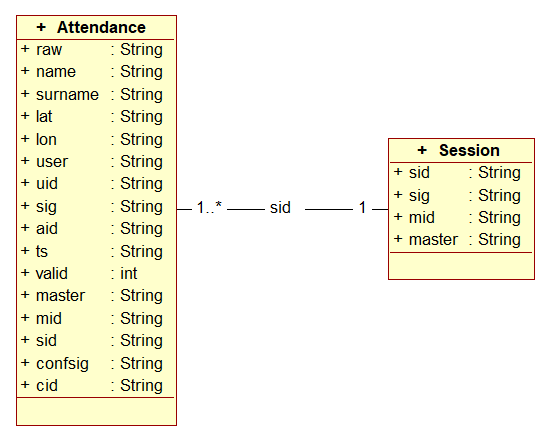
\includegraphics[width=0.6\textwidth]{material/classmodel}
    \caption{Dijagram klasa SPIM i SESS objekata}
\end{figure}
\begin{description}[align=right,labelwidth=2cm,noitemsep]
    \item [raw] serijalizirana string JSON verzija objekta
    \item [name] ime studenta
    \item [surname] prezime studenta
    \item [lat] geografska širina student
    \item [lon] geografska dužina student
    \item [user] ZAMGER korisničko ime studenta
    \item [uid] User ID - SHA2 hex hash javnog ključa studenta
    \item [sig] hex potpis SPIM-a (user:lat:lot:ts)
    \item [aid] Attendance ID - hex SHA2 hash \texttt{sig} potpisa
    \item [ts] vrijeme na studentovom uređaju
    \item [valid] validation cache
    \item [master] ZAMGER korisničko ime profesora
    \item [mid] Master ID - SHA2 hex hash javnog ključa profesora
    \item [sid] Session ID - identifikator profesorove sesije
    \item [confsig] Master Conf. profesorov hex potpis (sid:aid)
    \item [cid] Confirmation ID - SHA2 hex hash confsig-a
\end{description}

\subsection{SESS paket}
Dodatno se za SESS objekat prilikom finaliziranja sesije na LAPI serveru vrši prikupljanje svih CID potpisa koji pripadaju datoj sesiji, te se CID vrijednosti ulančane hronološkim redoslijedom potpisuju LAPI ključem koji se nalazi samo na LAPI hardverskom uređaju, stoga je sigurnost LAPI servera od ključne važnosti za sigurnost ukupnog sistema. Ovako potvrđena sesija ne može biti naknadno mijenjana, lažirana ili porečena izvan LAPI izvršnog okruženja.